\documentclass[border=10pt]{standalone}
\usepackage{tikz}
\usetikzlibrary{arrows.meta}
\begin{document}
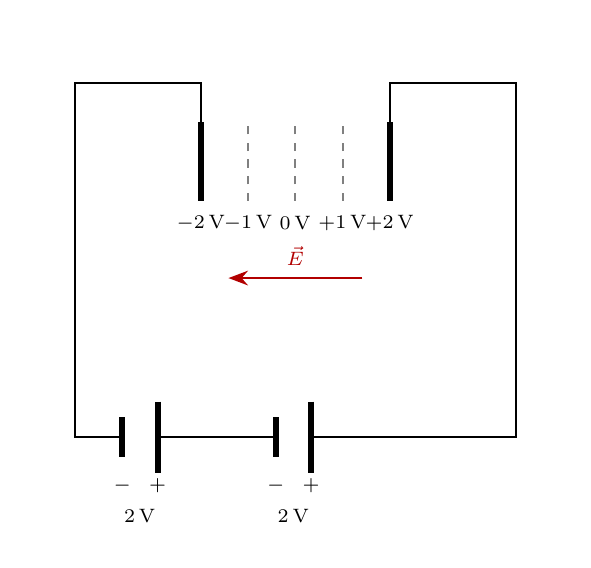
\begin{tikzpicture}[>=Stealth, scale=1.0, every node/.style={font=\scriptsize}]
  \useasboundingbox (-3.4,-3.3) rectangle (3.4,3.2);
  % parallel plates
  \draw[line width=2.2pt] (-1.2,1.0) -- (-1.2,2.0);
  \draw[line width=2.2pt] (1.2,1.0) -- (1.2,2.0);
  % equipotential lines
  \draw[dashed, line width=0.7pt, gray] (-0.6,1.0) -- (-0.6,2.0);
  \draw[dashed, line width=0.7pt, gray] (0,1.0) -- (0,2.0);
  \draw[dashed, line width=0.7pt, gray] (0.6,1.0) -- (0.6,2.0);
  % equipotential labels
  \node at (-1.2,0.72) {$-2\,\mathrm{V}$};
  \node at (-0.6,0.72) {$-1\,\mathrm{V}$};
  \node at (0,0.72) {$0\,\mathrm{V}$};
  \node at (0.6,0.72) {$+1\,\mathrm{V}$};
  \node at (1.2,0.72) {$+2\,\mathrm{V}$};
  % field direction (high -> low potential, right to left)
  \draw[->, line width=0.9pt, red!70!black] (0.85,0.02) -- (-0.85,0.02) node[midway, above, yshift=0.03cm] {$\vec{E}$};
  % wires
  \draw[line width=0.9pt] (-1.2,2.0) -- (-1.2,2.5) -- (-2.8,2.5) -- (-2.8,-2.0) -- (-2.2,-2.0);
  \draw[line width=0.9pt] (-1.75,-2.0) -- (-0.25,-2.0);
  \draw[line width=0.9pt] (0.2,-2.0) -- (2.8,-2.0) -- (2.8,2.5) -- (1.2,2.5) -- (1.2,2.0);
  % battery 1: - at x=-2.2, + at x=-1.75
  \draw[line width=2.2pt] (-2.2,-1.75) -- (-2.2,-2.25);
  \draw[line width=2.2pt] (-1.75,-1.55) -- (-1.75,-2.45);
  % battery 2: - at x=-0.25, + at x=0.2
  \draw[line width=2.2pt] (-0.25,-1.75) -- (-0.25,-2.25);
  \draw[line width=2.2pt] (0.2,-1.55) -- (0.2,-2.45);
  % terminal labels
  \node at (-2.2,-2.62) {$-$};
  \node at (-1.75,-2.62) {$+$};
  \node at (-0.25,-2.62) {$-$};
  \node at (0.2,-2.62) {$+$};
  \node at (-1.975,-3.0) {$2\,\mathrm{V}$};
  \node at (-0.025,-3.0) {$2\,\mathrm{V}$};
\end{tikzpicture}
\end{document}
